\section{问题三的建模与求解(23华中赛B题问题3示例)}



\subsection{数据预处理}

\subsubsection{数据清洗与特征编码}

本问要求对根据用药信息和患者信息对给药后 3 分钟以内的 IPI 数据进行预测,通过观察附件2发现只需要提取出IPI005、IPI1、IPI015、IPI2、IPI025、IPI3的相关数据,并从原始数据集中筛选出了需要的特征作为特征空间——包括性别、年龄、身高、体重、有无手术史、是否吸烟、是否酗酒、镇静药名称、镇静药诱导剂量、有无追加镇静、镇静药总剂量、镇痛药总剂量。

与上文数据预处理类似地,基于Pandas查找缺失值并删除一些对模型预测没有意义的特征,包括手术说明、既往史说明、ASA评分等,之后删除少量含有缺失值的行。对特征空间中的数值特征进行特征缩放中的数据归一化,以消除其量纲;对分类特征进行编码以转化为离散特征——这些特征包括性别、有无手术史等。

\subsubsection{数据降维}

由于数据集中有大量的分类特征导致数据集整体较为离散,模型难以充分提取特征,且容易过拟合。使用主成分分析法对处理后数据进行降维,当前数据共有14列,通过将方差解释比例可视化可得下图:

\begin{figure}[H] % 这个H不要动!
	\centering % 不要动!
	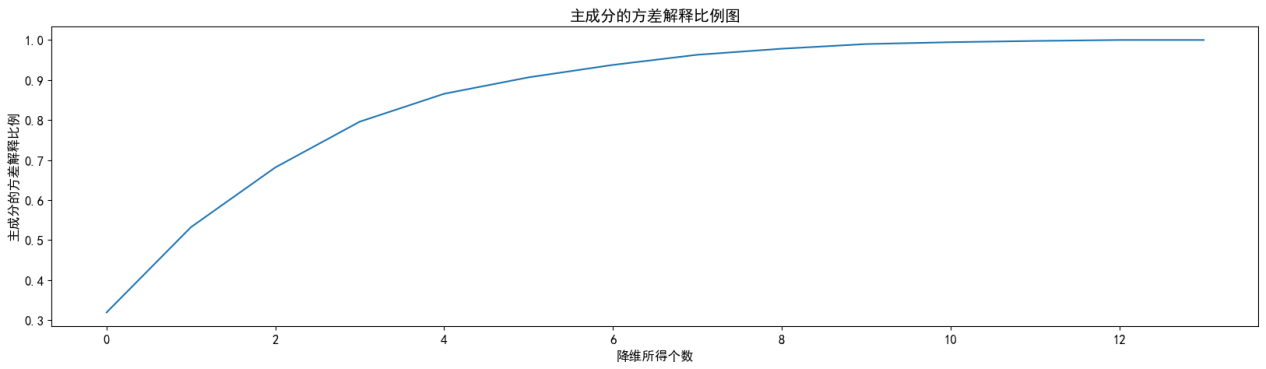
\includegraphics[width=0.95\textwidth]{8.png} 
	\caption{累积方差解释比例图} 
	\label{Fig.main8} 
\end{figure}

通过上图发现前四个主成分即可表示样本80\%的信息,因此保留了4个主成分,对4个主成分特征重新导入到数据集,便于后面利用监督学习中的回顾方法。

\subsection{岭回归与支持向量机回归的加权平均预测}


\subsubsection{模型建立}

\textbf{(一)岭回归模型}

\begin{enumerate}
	\item \textbf{岭回归}
	
	设有一个线性回归模型:
	
	\begin{equation}
		y=\overrightarrow{X}\overrightarrow{\beta }+\overrightarrow{\varepsilon }.
	\end{equation}
	其中,$\overrightarrow{X}$是$n\times p$的自变量矩阵,$\overrightarrow{\beta }$是$p$维系数向量,$y$是$n$维因变量向量,$\overrightarrow{\varepsilon }$是$n$维误差向量。
	
	引入L2正则化项后,岭回归的目标函数为:
	
	\begin{equation}
		\underset{\overrightarrow{\beta }}{\mathop{\min }}\,\left\{ \sum\limits_{i=1}^{n}{{{\left( {{y}_{i}}-\overrightarrow{x}_{i}^{T}\overrightarrow{\beta } \right)}^{2}}+\lambda \sum\limits_{j=1}^{p}{\overrightarrow{\beta }_{j}^{2}}} \right\}.
	\end{equation}
	其中,$\lambda$是正则化强度超参数,控制正则化项的权重大小。岭回归的解可以用闭式解表达式表示:
	
	\begin{equation}
		\widehat{\overrightarrow{\beta }}={{\left( {{\overrightarrow{X}}^{T}}\overrightarrow{X}+\lambda \overrightarrow{I} \right)}^{-1}}{{\overrightarrow{X}}^{T}}y.
	\end{equation}
	
	其中,$\overrightarrow{I}$是$p\times p$的单位矩阵。当$\lambda =0$时,岭回归就退化成了普通的线性回归;当$\lambda$取值较大时,正则化项的影响就越大,模型的系数就越接近于0。
	
	
	
	\item \textbf{支持向量机模型}
	
	对于数据集$D=\left\{ \left( {{\overrightarrow{x}}_{1}},{{y}_{1}} \right),\left( {{\overrightarrow{x}}_{2}},{{y}_{2}} \right),\cdots ,\left( {{\overrightarrow{x}}_{m}},{{y}_{m}} \right) \right\},$ ,得到一个回归模型$f\left( \overrightarrow{x} \right)$与$y$尽可能接近.SVR问题可形式化为:
	
	\begin{equation}
		f\left( \overrightarrow{x} \right)={{\overrightarrow{\omega }}^{T}}\Phi \left( \overrightarrow{x} \right)+b.
	\end{equation}
	
	\begin{equation}
		\overrightarrow{\omega }=\sum\limits_{i=1}^{m}{\left( {{\widehat{\alpha }}_{i}}-{{\alpha }_{i}} \right)\Phi \left( {{\overrightarrow{x}}_{i}} \right)}.
	\end{equation}
	
	\begin{equation}
		f\left( \overrightarrow{x} \right)=\sum\limits_{i=1}^{m}{\left( {{\widehat{\alpha }}_{i}}-{{\alpha }_{i}} \right)\kappa \left( \overrightarrow{x},{{\overrightarrow{x}}_{i}} \right)}+b.
	\end{equation}
	其中$\kappa \left( {{\overrightarrow{x}}_{i}},{{\overrightarrow{x}}_{j}} \right)=\Phi {{\left( {{\overrightarrow{x}}_{i}} \right)}^{T}}\Phi \left( {{\overrightarrow{x}}_{j}} \right)$为核函数.$\overrightarrow{\omega },b$为模型参数,${{\widehat{\alpha }}_{i}}\ge 0,{{\alpha }_{i}}\ge 0$是拉格朗日乘子.利用高斯核函数求解,公式为:
	
	\begin{equation}
		\kappa \left( {{\overrightarrow{x}}_{i}},{{\overrightarrow{x}}_{j}} \right)=\exp \left( -\frac{\left\| {{\overrightarrow{x}}_{i}}-{{\overrightarrow{x}}_{j}} \right\|}{2{{\sigma }^{2}}} \right).
	\end{equation}
	
\end{enumerate}





\subsubsection{模型求解}

首先基于Scikit-Learn建立三分钟内各时间点的IPI数值的两种预测模型——岭回归模型和SVR模型,设定岭回归模型在$i$样本的预测值为${{h}_{1}}({{\overrightarrow{x}}_{i}})$,SVR模型的预测值为${{h}_{2}}({{\overrightarrow{x}}_{i}}),i=1,2,\cdots ,m$,构建集成学习器$H$包含两个基学习器{${{h}_{1}},{{h}_{2}}$}。


对于题目中由已知的数据集进行建模,分别需要对六个标签——IPI005、IPI1、IPI015、IPI2、IPI025以及IPI3进行回归分析。加权平均法是一种常见的回归任务的模型融合方法,利用加权平均法进行结合,其中原理如下:

\begin{equation}
	{{\omega }_{i}}=\frac{MS{{E}_{i}}}{MS{{E}_{1}}+MS{{E}_{2}}},i=1,2.
\end{equation}


\begin{equation}
	H(\overrightarrow{x})=\frac{1}{2}\sum\limits_{i=1}^{2}{{{\omega }_{i}}{{h}_{i}}(\overrightarrow{x})}.
\end{equation}
其中,${{\omega }_{1}},{{\omega }_{2}}$分别表示两个模型的权重,通过计算两种模型集成后组成的最优模型$H(\overrightarrow{x})$。

对于两个基学习器和基于加权平均法的融合模型,本文分别在测试集上进行测试,基于MAE和MSE对模型泛化能力进行评价,所得如下:

\begin{table}[H]
	\centering  
	\caption{三种模型在测试集上的测试评价}
	\begin{tabular}{c c c c}  
		\toprule[1.5pt]  
		标签名称 & 模型 & MAE & MSE  \\  
		\midrule[1pt]    
		\multirow{3}{*}{IPI005} & 岭回归   & 0.1447	& 0.0423    \\ 
		& SVR      & 0.1418	& 0.0417    \\
		& 模型融合 & 0.1432	& 0.0419    \\
		\multirow{3}{*}{IPI1}   & 岭回归   & 0.2376	& 0.1020    \\ 
		& SVR      & 0.2272	& 0.1153    \\
		& 模型融合 & 0.2322	& 0.1066    \\
		\multirow{3}{*}{IPI015} & 岭回归   & 0.3669	& 0.1630	\\ 
		& SVR      & 0.3567	& 0.1808	\\
		& 模型融合 & 0.3570	& 0.1651	\\
		\multirow{3}{*}{IPI2}   & 岭回归   & 0.2666	& 0.1103	\\ 
		& SVR      & 0.2363	& 0.1174	\\
		& 模型融合 & 0.2509	& 0.1101	\\
		\multirow{3}{*}{IPI025} & 岭回归   & 0.1680	& 0.0679	\\ 
		& SVR      & 0.1663	& 0.0682	\\
		& 模型融合 & 0.1671	& 0.0678	\\
		\multirow{3}{*}{IPI3}   & 岭回归   & 0.1810	& 0.0798	\\ 
		& SVR      & 0.1788	& 0.0810	\\
		& 模型融合 & 0.1797	& 0.0800    \\
		\toprule[1.5pt]  
	\end{tabular}  
\end{table} 

分析上表可知,基于三种模型在测试集上的评价指标,对于这六种标签预测评价指标都接近0,说明这三种模型的预测效果都十分优良。从标签种类分析,可以发现对于标签IPI005的预测效果最佳,对于标签IPI015的预测效果最差。不同标签预测效果整体上的优良性从最优到优的排序为IPI005、IPI025、IPI3、IPI1、IPI2、IPI015。

分析三种模型发现无论是岭回归模型还是SVR模型都不能保证是性能最优,而将模型融合可以弥补单个模型的不足,提高准确率。同时提升模型的鲁棒性,降低由于数据的随机性导致的模型波动,得到的预测结果更准确,泛化能力更强,模型稳定性更强。模型融合是提高预测准确性、提高模型鲁棒性、降低模型波动性的一种有效方法。



\subsubsection{灵敏度分析}

为了评估两个不同的模型(Ridge回归和支持向量机)对输入数据的敏感性,这里通过施加一些高斯噪声(从0到0.5的比例),原理为

\begin{equation}
	f\left( x \right)=\frac{1}{\sigma \sqrt{2\pi }}{{e}^{-\frac{{{\left( x-\mu  \right)}^{2}}}{2{{\sigma }^{2}}}}}.
\end{equation}
其中,$x$表示随机变量的取值,$\mu$表示期望值,$\sigma$表示标准差。改变测试数据集的特征,来模拟模型的偏差,以确定模型的鲁棒性。然后根据分段函数:

\begin{equation}
	erro{{r}_{ij}}=\left\{ \begin{matrix}
		0  \\
		{{\overline{y}}_{ij}}+f({{x}_{j}})  \\
	\end{matrix} \right.\begin{matrix}
		,\left( 0,c \right)  \\
		,\left( c,0.5 \right)  \\
	\end{matrix}
\end{equation}
其中$\overline{y}_{ij}$为第$i$个特征的第$j$个的样本值,$f({{x}_{j}})$表示加入的高斯噪声,$c$表示噪音阈值。重新预测,并计算预测结果与真实结果之间的均方误差。下文以IPI3为例对模型灵敏度进行分析(其余见附件),得到数据可视化图如下所示:

\begin{figure}[H] % 这个H不要动!
	\centering % 不要动!
	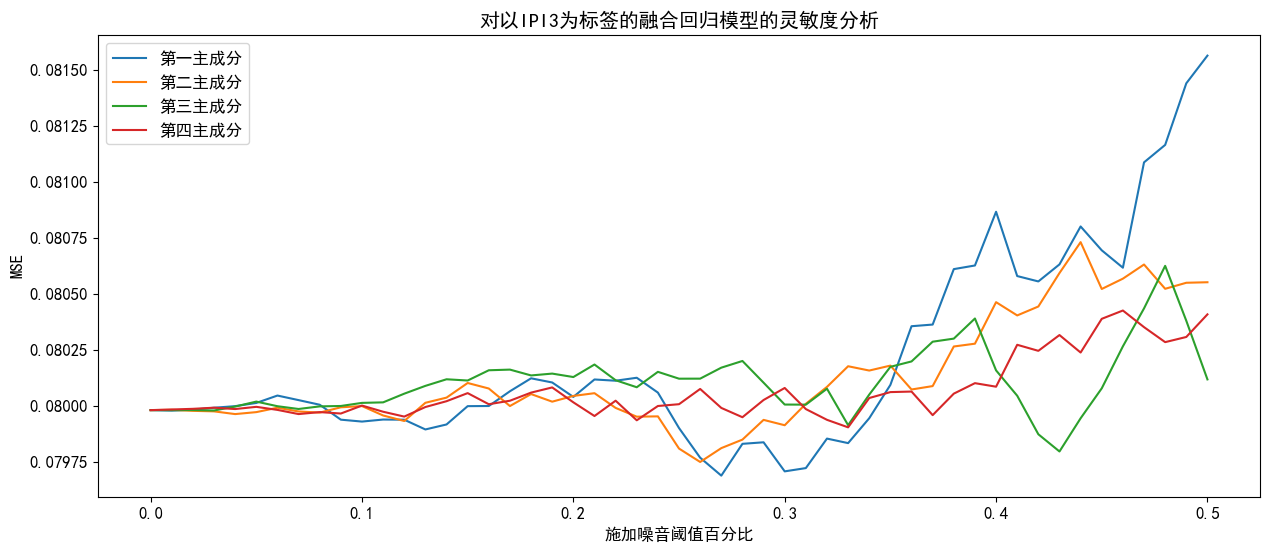
\includegraphics[width=0.95\textwidth]{9.png} 
	\caption{对以IPI3为标签的融合回归模型的灵敏度分析} 
	\label{Fig.main9} 
\end{figure}

从上图可以看出,对第一主成分、对第二主成分、对第三主成分、对第四主成分分别不断施加噪音,可以直观地看出MSE(均方差)值在这个区间波动,四个特征在施加噪音百分比在30\%以内时MSE均无明显波动,说明该模型具有一定的可靠性和稳定性性能优良。另外五个标签的灵敏度分析图详见附录A。
